\begin{lstlisting}[float=p,label=lst:csdg-simple,
  caption={Program using load-time variability resulting in the SDG in \autoref{fig:csdg-simple}}]
class Main {
  static final boolean c0 = getConfiguration("c0");
  static final boolean c1 = getConfiguration("c1");
  
  public static void main(String[] args) {
    int res = 0;
    if(c0) {
      res = foo();
      return;
    } else if(c1)
      res = foo();
    System.out.println(res);
  }
  
  private static int foo() {
    if(!c1)
      (@@)`return 1`;
    return 0;
  }
}
\end{lstlisting}

\begin{figure}[p]
  \centering
    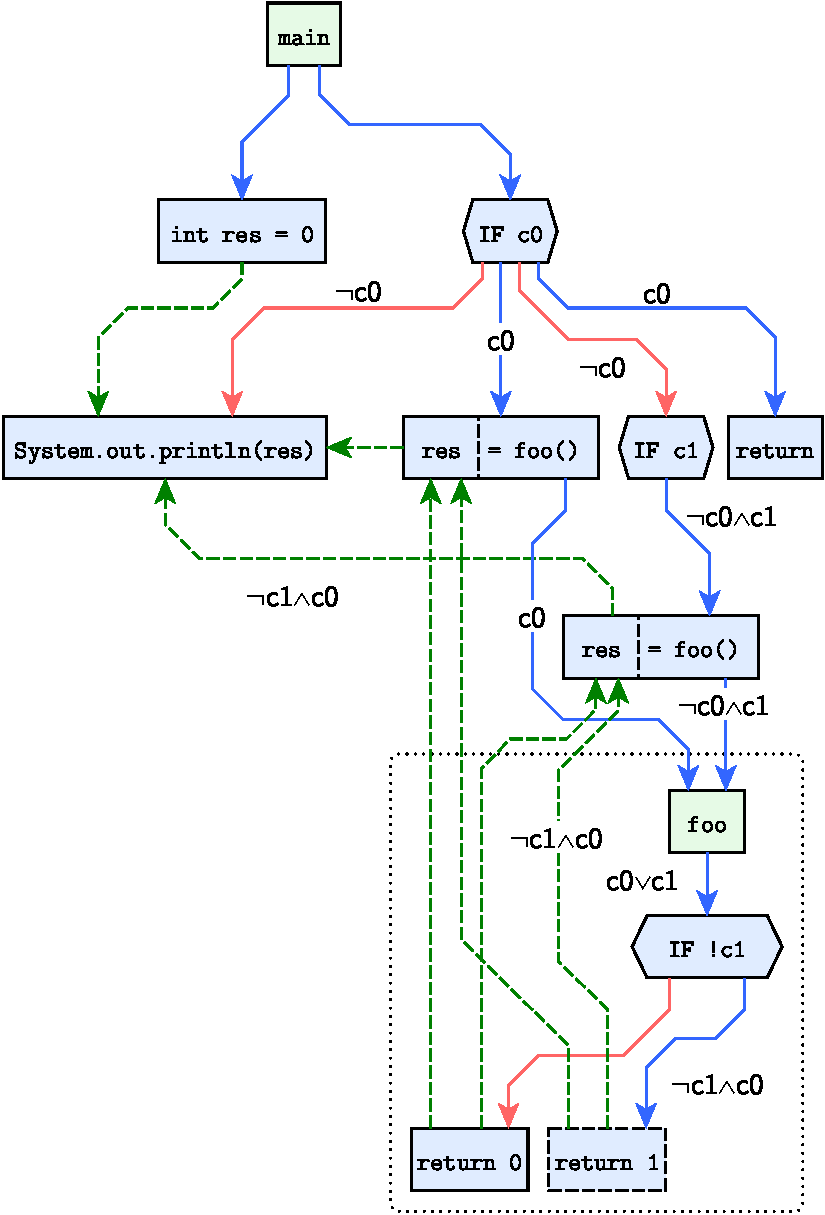
\includegraphics[scale=0.6]{sdgs/simple-csdg}
  \caption{Simplified CSDG for the sample program in \autoref{lst:csdg-simple}}
  \label{fig:csdg-simple}
\end{figure}
